%%%%%%%%%%%%%%%%%%%%%%%%%%%%%%%%%%%%%%%%%%%%%%%%%%%%%%%%%%%%%%%%%%%%%%%%%%%%%%%%%%%%%%%%%
% Khóa luận tốt nghiệp/Tiểu luận 
% LaTeX Template
% Phiên bản 1.0 (tạo ra ngày 05/10/2022)
% Edited &Modified by VietNC ngày 12/12/2022
%
% Template này có thể được download tại:
% https://github.com/vietnc/HUS-template
% https://github.com/cpc1996/HUS-Dissertation-Template
% 
%
% Phiên bản 1.0 được chỉnh sửa bởi:
% Công Phương Cao (congphuongcao_t59@hus.edu.vn)
% Nguyễn Cảnh Việt (vietncp@gmail.com)
% Nguyễn Tiến Cường (ngtiencuong@gmail.com)
%
% Template được tham khảo từ một phiên bản template của:
% Steve Gunn (http://users.ecs.soton.ac.uk/srg/softwaretools/document/templates/)
% Sunil Patel (http://www.sunilpatel.co.uk/thesis-template/)
%
%%%%%%%%%%%%%%%%%%%%%%%%%%%%%%%%%%%%%%%%%%%%%%%%%%%%%%%%%%%%%%%%%%%%%%%%%%%%%%%%%%%%%%%%%
%----------------------------------------------------------------------------------------
%	(KHÔNG CHỈNH SỬA PHẦN NÀY)
%
%	PHẦN 1: CÁC PACKAGE CƠ BẢN VÀ CÁC TÙY CHỈNH VĂN BẢN
%----------------------------------------------------------------------------------------
%----------------------------------------------------------------------------------------
%	(KHÔNG CHỈNH SỬA PHẦN NÀY)
%
%	PHẦN 1: CÁC PACKAGE CƠ BẢN VÀ CÁC TÙY CHỈNH VĂN BẢN
%----------------------------------------------------------------------------------------

\documentclass[
12pt,
oneside,
english,
doublespacing,
nolistspacing,
liststotoc,
parskip,
headsepline,
chapterinoneline,
]{MastersDoctoralThesis}

% \usepackage[utf8]{inputenc} 
\usepackage[utf8]{vietnam} 
%\usepackage[T1]{fontenc}

\usepackage{mathptmx}
\usepackage{amsmath}
\usepackage{textcomp}
\allowdisplaybreaks

%https://www.overleaf.com/learn/latex/Biblatex_citation_styles
%\usepackage[backend=bibtex,style=authoryear,natbib=true]{biblatex}
\usepackage[backend=bibtex,style=numeric,citestyle=ieee,natbib=true]{biblatex}

\addbibresource{main.bib}

\usepackage[autostyle=true]{csquotes}


%----------------------------------------------------------------------------------------
%	PHẦN 2: CÁC PACKAGE BỔ TRỢ THÊM VÀO TRONG QUÁ TRÌNH BIÊN SOẠN
%----------------------------------------------------------------------------------------

\RequirePackage{setlst}		% Liệt kê/trích dẫn code

\usepackage{multirow}
\usepackage{subfigure}
\usepackage[fontsize=13pt]{scrextend}

%https://www.sascha-frank.com/latex-font-size.html
%https://tex.stackexchange.com/questions/103286/how-to-change-section-subsection-font-size
\usepackage{titlesec}

\titleformat{\section}
{\normalfont\fontsize{13}{13}\bfseries}{\thesection}{1em}{}

\titleformat{\subsection}
{\normalfont\fontsize{13}{13}\bfseries\itshape}{\thesubsection}{1em}{}

%https://tex.stackexchange.com/questions/351961/how-to-indent-code-in-beginverbatim
\usepackage{fancyvrb} 		% Fancy Verbatim
\fvset{tabsize=4,vspace=0pt,fontsize=\footnotesize}

\usepackage{longtable} 		% Bảng dài - Long table

\usepackage[figuresright]{rotating} % Bảng ngang - Sideways table
\usepackage{tabularx}

\usepackage{fontawesome5} 	% Các biểu tượng, ký hiệu đặc biệt

\usepackage{tikz} 			% Vẽ hình
\usepackage{indentfirst}
\setlength{\parindent}{0.5cm}	%Thut dau dong cho doan van
\setlength{\parskip}{1.4ex plus 0.5ex minus 0.3ex}		% Tạo khoảng trống giữa 2 đoạn văn %spacing between two paragraph

\usetikzlibrary{calc}

%----------------------------------------------------------------------------------------
%	PHẦN 3: THÔNG TIN VỀ Khóa luận tốt nghiệp/Tiểu luận (THESIS INFORMATION)
% 	Điền thông tin của các bạn trong file(2.thesis-information) này 
%----------------------------------------------------------------------------------------
%----------------------------------------------------------------------------------------
%	PHẦN 3: THÔNG TIN VỀ Khóa luận tốt nghiệp/Tiểu luận (THESIS INFORMATION)
%----------------------------------------------------------------------------------------
\author{VI ANH QUÂN\\
		TRẦN ANH MINH\\
		NGUYỄN NHẬT TÙNG\\ 
		NGUYỄN TIẾN ĐẠT
} 			% Ví dụ: "Nguyễn Thị Thu Thảo"
\thesistitle{MÔ HÌNH SINH TẢ ẢNH DỰA TRÊN CẢM XÚC		 } % Ví dụ: "Nghiên cứu chế tạo và tính chất quang học của vật liệu nano LaF3:Sm3+"

\supervisor {TS. Phạm Tiến Lâm} 	% Ví dụ: "PGS. TS. Nguyễn Ngọc Long"

\field{Ngành Kĩ thuật Điện tử và Tin học} 					% Ví dụ: "Ngành Vật lý", "Ngành Hóa học", v.v.
\program{Chương trình đào tạo chuẩn} 			% Ví dụ: "Chương trình đào tạo chuẩn", "Chương trình đào tạo cử nhân tài năng", v.v.
\doctype{Báo cáo kết thúc môn Machine Learning} % Điền vào đây: "Khóa luận tốt nghiệp đại học hệ chính quy" hoặc "Tiểu luận"

\university{\href{http://hus.vnu.edu.vn}{TRƯỜNG ĐẠI HỌC KHOA HỌC TỰ NHIÊN}}
\department{\href{http://hus.vnu.edu.vn/gioi-thieu/co-cau-to-chuc/khoa-truc-thuoc/khoa-vat-ly.html}{KHOA VẬT LÝ}}

\AtBeginDocument{
	\hypersetup{pdftitle=\ttitle}
	\hypersetup{pdfauthor=\authorname}
}

%----------------------------------------------------------------------------------------------------------------------------------------
\begin{document}
\lstset{style=codeC}	% Thiết lập ngôn ngữ C/C++ là ngôn ngữ mặc định cho phần liệt kê souce code của cả bài
\frontmatter 			% Sử dụng hệ thống đánh số La Mã (i, ii, iii, iv...) cho những trang trước phần mục lục
\pagestyle{plain} 
%----------------------------------------------------------------------------------------
%	(KHÔNG CHỈNH SỬA PHẦN NÀY)%
%	PHẦN 4: TRANG TIÊU ĐỀ/TRANG BÌA (TITLE PAGE)
%----------------------------------------------------------------------------------------
% TRANG BÌA CHÍNH:
%----------------------------------------------------------------------------------------
%	(KHÔNG CHỈNH SỬA PHẦN NÀY)
%
%	Phần 6: TRANG TIÊU ĐỀ/TRANG BÌA (TITLE PAGE)
%----------------------------------------------------------------------------------------

% TRANG BÌA CHÍNH:
\begin{titlepage}
	\begin{tikzpicture}[overlay,remember picture]
		\draw [line width=3pt]
		($ (current page.north west) + (2.0cm,-2.0cm) $)
		rectangle
		($ (current page.south east) + (-1.5cm,1.8cm) $);
		\draw [line width=1pt]
		($ (current page.north west) + (2.15cm,-2.15cm) $)
		rectangle
		($ (current page.south east) + (-1.65cm,1.95cm) $); 
	\end{tikzpicture}
	\begin{center}
		
		\vspace{-.04\textheight}
%		\noindent\scshape 			% By CPC
		\noindent 			% Edit by VietNC
		\large \, \href{https://www.vnu.edu.vn/home/}{ĐẠI HỌC QUỐC GIA HÀ NỘI}\\
		\vspace{-0.25cm}{\large \MakeUppercase \univname}\\
		\vspace{-0.25cm}{\large \bfseries \MakeUppercase \deptname}\\[0.5cm]
		
\includegraphics{Logo/Logo_HUS_notext_nocolor}
		
		\vspace{1.0cm}
		
		{\large \MakeUppercase \authorname}
		
		\vspace{2.5cm}
		
		{\Large \bfseries \MakeUppercase\ttitle\par}
		
		\vspace{2.5cm}
		
		{\normalsize \docname\\ \fieldname\\ (\progname)\\}
		
		\vfill
		
		\textbf{Hà Nội - \the\year{}}
	\end{center}
\end{titlepage}


% TRANG BÌA PHỤ:
%----------------------------------------------------------------------------------------
%	(KHÔNG CHỈNH SỬA PHẦN NÀY)
%
%	Phần 6: TRANG TIÊU ĐỀ/TRANG BÌA (TITLE PAGE)
%----------------------------------------------------------------------------------------

% TRANG BÌA PHỤ:
\begin{titlepage}
	\begin{tikzpicture}[overlay,remember picture]
		\draw [line width=3pt]
		($ (current page.north west) + (2.0cm,-2.0cm) $)
		rectangle
		($ (current page.south east) + (-1.5cm,1.8cm) $);
		\draw [line width=1pt]
		($ (current page.north west) + (2.15cm,-2.15cm) $)
		rectangle
		($ (current page.south east) + (-1.65cm,1.95cm) $); 
	\end{tikzpicture}
	\begin{center}
		
		\vspace{-.04\textheight}
%		\noindent\scshape    % By CPC
		\noindent                  % Edit by VietNC
		\large \, \href{https://www.vnu.edu.vn/home/}{ĐẠI HỌC QUỐC GIA HÀ NỘI}\\
		\vspace{-0.25cm}{\large \MakeUppercase \univname}\\
		\vspace{-0.25cm}{\large \bfseries \MakeUppercase \deptname}\\[0.5cm]
		
\includegraphics{Logo/Logo_HUS_notext}
		
		\vspace{1.0cm}
		
		{\large \MakeUppercase \authorname}
		
		\vspace{2.5cm}
		
		{\Large \bfseries \MakeUppercase\ttitle\par}
		
		\vspace{1.5cm}
		
		{\normalsize \docname\\ \fieldname\\ (\progname)\\}
		
		\vspace{1.0cm}
		\begin{minipage}[t]{0.49\textwidth}
			\centering
			\begin{flushright} \large \bfseries
				Giảng viên hướng dẫn:\;
			\end{flushright}
		\end{minipage}
		\begin{minipage}[t]{0.5\textwidth}
			\begin{flushleft} \large \bfseries
				\supname\\				
			\end{flushleft}
		\end{minipage}
		
		\vfill
		
		\textbf{Hà Nội - \the\year{}}
	\end{center}
\end{titlepage}


%----------------------------------------------------------------------------------------
%	PHẦN 5: DANH NGÔN (QUOTES)
%----------------------------------------------------------------------------------------
%\vspace*{0.2\textheight}

%\noindent\enquote{\itshape 
%	Cái tôi và sự hiểu biết tỷ lệ nghịch với nhau. Hiểu biết càng nhiều cái tôi càng bé. Hiểu biết càng ít, cái tôi càng to.
%}\bigbreak

%\hfill Albert Einstein
%----------------------------------------------------------------------------------------
%	PHẦN 6: LỜI CẢM ƠN (ACKNOWLEDGEMENTS)
%	Các bạn ghi lời cảm ơn vào file(5.ack) này.
%----------------------------------------------------------------------------------------
%----------------------------------------------------------------------------------------
%	PHẦN 6: LỜI CẢM ƠN (ACKNOWLEDGEMENTS)
%----------------------------------------------------------------------------------------

\begin{acknowledgements}
	\addchaptertocentry{\acknowledgementname}
	\thispagestyle{empty}
	
	Trong quá trình học tập môn Machine learning, chúng em đã nhận được sự giúp đỡ nhiệt tình của thầy Phạm Tiến Lâm và thầy Đặng Văn Báu. Thầy đã cung cấp cho chúng em những kiến thức vô cùng quan trọng để phục vụ trong quá trình học tập và nghiên cứu. Chúng em rất trân trọng khoảng thời gian cùng thầy nghiên cứu môn học vô cùng thú vị này. 
	
	Do những hạn chế về kiến thức, dự án này của chúng em cũng không tránh khỏi những thiếu sót. Chúng em rất mong nhận được sự đóng góp, phê bình của các thầy để đề tài của chúng em được hoàn thiện hơn. Cuối cùng em xin kính chúc thầy nhiều sức khỏe, thành công và hạnh phúc.
	
	Chúng em xin chân thành cảm ơn!
	
\end{acknowledgements}

\begin{flushright}
	\textit{Hà Nội, tháng 6 năm 2023}\hspace{0.5cm}
	\vspace{0.1cm}\\
	\textbf{Sinh viên}\hspace{2cm}
	\vspace{2cm}
\end{flushright}
%----------------------------------------------------------------------------------------
%	(KHÔNG CHỈNH SỬA PHẦN NÀY)
%
%	PHẦN 7: MỤC LỤC (LIST OF CONTENTS/FIGURES/TABLES PAGES)
%	ĐẶT KHOẢNG CÁCH GIŨA CÁC TIÊU ĐỀ CỦA PHẦN 7
%----------------------------------------------------------------------------------------
\begin{spacing}{1.15}
	\tableofcontents 	% In ra mục lục chính
\end{spacing}

\begin{spacing}{1.15}
	\listoffigures 		% In ra danh sách hình vẽ
\end{spacing}

%\begin{spacing}{1.15}
%	\listoftables		% In ra danh sách bảng
%\end{spacing}

%----------------------------------------------------------------------------------------
%	PHẦN 8: DANH SÁCH TÊN VIẾT TẮT (ABBREVIATIONS)
%
%	Các từ viết tắt các bạn ghi ở đây
%----------------------------------------------------------------------------------------
%\begin{abbreviations}{ll} % Thêm danh sách tên viết tắt (dưới dạng một bảng có 2 cột)
%
%\textbf{TVT} & \textbf{T}ên \textbf{V}iết \textbf{T}ắt\\
%\textbf{ĐTĐ} & \textbf{Đ}ặt (nó) \textbf{T}ại \textbf{Đ}ây\\
%
%\end{abbreviations}
%----------------------------------------------------------------------------------------
%	PHẦN 9: CÁC HẰNG SỐ VẬT LÝ/THÔNG SỐ KĨ THUẬT (PHYSICAL CONSTANTS/OTHER DEFINITIONS)
%----------------------------------------------------------------------------------------
%\begin{constants}{lr@{${}={}$}l} % Thêm danh sách các hằng số (dưới dạng một bảng có 3 cột)
%
%%	Lệnh \SI{}{} được cung cấp bởi gói siunitx, hãy đọc tài liệu hướng dẫn để biết cách sử dụng nó
%
%%	Tên hằng số 	 & $Biểu tượng$	& $Hằng số$ cùng với đơn vị\\
%	Vận tốc ánh sáng & $c_{0}$		& \SI{2.99792458e8}{\meter\per\second} (chính xác)\\
%
%\end{constants}
%----------------------------------------------------------------------------------------
%	PHẦN 10: DANH SÁCH KÝ HIỆU (SYMBOLS)
%----------------------------------------------------------------------------------------

%\begin{symbols}{lll} % Thêm danh sách các ký hiệu (dưới dạng một bảng có 3 cột)
%
%%   Ký hiệu	& Ý nghĩa		& Đơn vị \\
%	$a$		& khoảng cách	& \si{\meter} \\
%	$P$		& công suất		& \si{\watt} (\si{\joule\per\second}) \\
%
%	\addlinespace % Khoảng cách để phân biệt giữa ký hiệu Latin với ký hiệu La Mã
%
%	$\omega$ & tần số góc	& \si{\radian} \\
%
%\end{symbols}

%----------------------------------------------------------------------------------------
%	(KHÔNG CHỈNH SỬA PHẦN NÀY)
%
%	PHẦN 11: LỜI ĐỀ TẶNG (DEDICATION)
%----------------------------------------------------------------------------------------

%\dedicatory{Dành tặng/Dành cho/Gửi tới\ldots} 


%----------------------------------------------------------------------------------------
%	PHẦN 12: NỘI DUNG/CÁC CHƯƠNG Khóa luận tốt nghiệp/Tiểu luận (THESIS CONTENT - CHAPTERS)
%----------------------------------------------------------------------------------------

\mainmatter % Bắt đầu đánh số trang (1,2,3...)

\pagestyle{plain}

% Hãy thêm những chương (chapter) của khóa luận/tiểu luận vào thư mục Chapters
% Hãy bỏ chú thích những dòng nếu bạn đã bổ sung những chương vào

%% MỞ ĐẦU (LỜI MỞ ĐẦU - Chương 0)

\chapter*{MỞ ĐẦU} % Tên của chương
\addcontentsline{toc}{chapter}{MỞ ĐẦU} % Thêm tên chương vào mục lục

\label{Chapter0} % Để trích dẫn chương này ở chỗ nào đó trong bài, hãy sử dụng lệnh \ref{Chapter0} 

Hiện nay, Internet là một thứ đã rất phổ biến trên toàn thế giới. Những lợi ích của nó mang lại là không thể chối cãi: giải trí, cập nhật thông tin nhanh chóng, kết nối mọi người với nhau bất kể khoảng cách,.... Từ đó Internet of Thing (IoT), một công nghệ với cốt lõi là các tính năng của Internet, đã được ra đời. Với IoT, những vật dụng tưởng chừng vô tri như bóng đèn, quạt điện, tủ lạnh, xe máy, công tơ điện,... lại có thể giao tiếp, truyền tải thông tin với nhau. Để làm được điều đó thì không thể thiếu được các giao thức, thứ được ví như là các quy tắc giao tiếp chung trong thế giới IoT. 

Trên thực tế, đã có rất nhiều hệ thống IoT được thương mại hóa, áp dụng trong tất cả các lĩnh vực của đời sống. Tất cả các hệ thống này đều có một yêu cầu chung là truyền tải thông tin nhanh chóng, an toàn và ít xảy ra lỗi.

Xuất phát từ yêu cầu đó, đề tài "\textbf{Giao thức MQTT và các ứng dụng trong IoT}" đã được tôi lựa chọn. Tiểu luận này sẽ nghiên cứu giao thức MQTT, một giao thức được phát triển với mục đích truyền tải các thông tin nhanh chóng, có thể sử dụng kể cả khi kết nối mạng không ổn định. Dựa trên cơ sở đó áp dụng vào mô hình trao đổi dữ liệu nhiệt độ độ ẩm từ cảm biến DHT11 thông qua hai board điều khiển ESP8266.

Các phần chính của tiểu luận này bao gồm những phần sau:
\begin{itemize}
	\item {\textbf{Chương 1 - Tổng quan về Internet:}}
	Trong chương này sẽ trình bày các kiến thức liên quan tới Internet bao gồm lịch sử phát triển,các thành phần chính và cách vận hành.
	\item {\textbf{Chương 2 - Tổng quan về IoT và giao thức MQTT:}}
	Chương này trình bày tổng quan về IoT, các thành phần của nó. Tiếp đến là giới thiệu về giao thức MQTT, lí do nó được chọn là giao thức nghiên cứu trong tiểu luận lần này.
	\item {\textbf{Chương 3 - Thực nghiệm:}}
	Thông tin phần cứng, phần mềm được áp dụng sẽ được trình bày ở chương này. Cùng với đó là cách thiết kế hệ thống, sơ đồ hoạt động, thuật toán phần mềm.
	\item {\textbf{Kết luận:}}
	Cuối cùng là tổng kết lại kết quả thu được sau một thời gian nghiên cứu đề tài, những ứng dụng, hạn chế của mô hình và phương hướng giải quyết.
\end{itemize}
\chapter{MỞ ĐẦU} % Tên của chương

\label{Chapter1} % Để trích dẫn chương này ở chỗ nào đó trong bài, hãy sử dụng lệnh \ref{Chapter1} 

%----------------------------------------------------------------------------------------

% Định nghĩa một số lệnh cần thiết để điều chỉnh định dạng cho một số nội dung nhất định trong bài
\newcommand{\keyword}[1]{\textbf{#1}}
\newcommand{\tabhead}[1]{\textbf{#1}}
\newcommand{\code}[1]{\texttt{#1}}
\newcommand{\file}[1]{\texttt{\bfseries#1}}
\newcommand{\option}[1]{\texttt{\itshape#1}}

%----------------------------------------------------------------------------------------
Hiện nay trí tuệ nhân tạo là một xu hướng công nghệ trên toàn thế giới. Nó đã xuất hiện ở mọi nơi như là mạng xã hội, thiết bị điện tử, xe cộ, .... Xuất phát từ nhu cầu ngày càng cao của con người về sự tiện lợi, thông tin nhanh chóng thì mô hình nhận diện hành động con người cũng đã được ra đời.

Nhận diện hành động con người ở ảnh tĩnh có rất nhiều tiềm năng ứng dụng vào đời sống như là thiết bị hỗ trợ người khiếm thị, gán nhãn tự động, .... Một giải pháp trực tiếp cho vấn đề đó chính là từ hình ảnh sinh ra được văn bản mô tả chính xác ảnh đó với lời văn hợp lý. Tuy nhiên thử thách được đặt ra đó là con người có rất nhiều trạng thái hoạt động phức tạp khác nhau cùng với ngữ pháp mỗi loại ngôn ngữ là khác nhau. Chính vì vậy bài báo cáo này sẽ tập trung vào một số trạng thái cơ bản của con người và mô tả nó bằng tiếng Anh. Các mô hình Machine learning và Deep learning được sử dụng trong bài báo cáo này là CNN, RNN và LSTM. Đây là các mô hình rất phổ biến trên thế giới, được tin dùng trong việc xử lí ảnh và ngôn ngữ tự nhiên.
\chapter{TỔNG QUAN} % Tên của chương

\label{Chapter2} % Để trích dẫn chương này ở chỗ nào đó trong bài, hãy sử dụng lệnh \ref{Chapter1} 
\section{Dataset sử dụng}
Việc sử dụng nhiều dataset khác nhau cho phép đa dạng dữ liệu
đầu vào và kiểm tra được tính linh hoạt của mô hình trong nhiều trường hợp khác nhau.
\subsection{Emotional attitude captioning dataset}
Dataset sử dụng trong bài có 3840 ảnh khác nhau, được lấy từ IMDB dataset. Mỗi ảnh được gán nhãn với một số trạng thái như là "laughing", "flirting", "kissing", "angry", "happy", ...\cite{web:4}. 

\begin{figure}[h!]
	\centering
	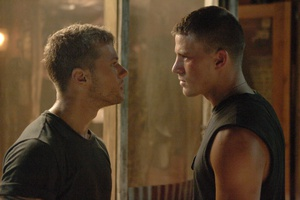
\includegraphics[width=10cm]{nm0000202_rm1918408960_1974-9-10_2008.jpg}
	\caption{Gán nhãn: Two guys are looking on each other.}
\end{figure} 
\subsection{Flickr8}
Dataset được lấy trên trang web Kaggle \cite{web:8}.

\section{Mô hình CNN}
CNN (Convolutional Neural Network) là một mô hình Deep learning để xử lí dữ liệu ở dạng lưới như là hình ảnh, được thiết kế để học một cách tự động và thích ứng với hệ thống phân cấp không gian của các tính năng, từ pattern thấp tới cao.\cite{yamashita2018convolutional}

Nó sử dụng một kĩ thuật đặc biệt gọi là tích chập (Convolution), một phép toán trên hai phương trình để đưa ra phương trình thứ ba mô tả cách hình dạng của một phương trình bị thay đổi bởi phương trình còn lại.\cite{web:2}

\begin{figure}[h!]
	\centering
	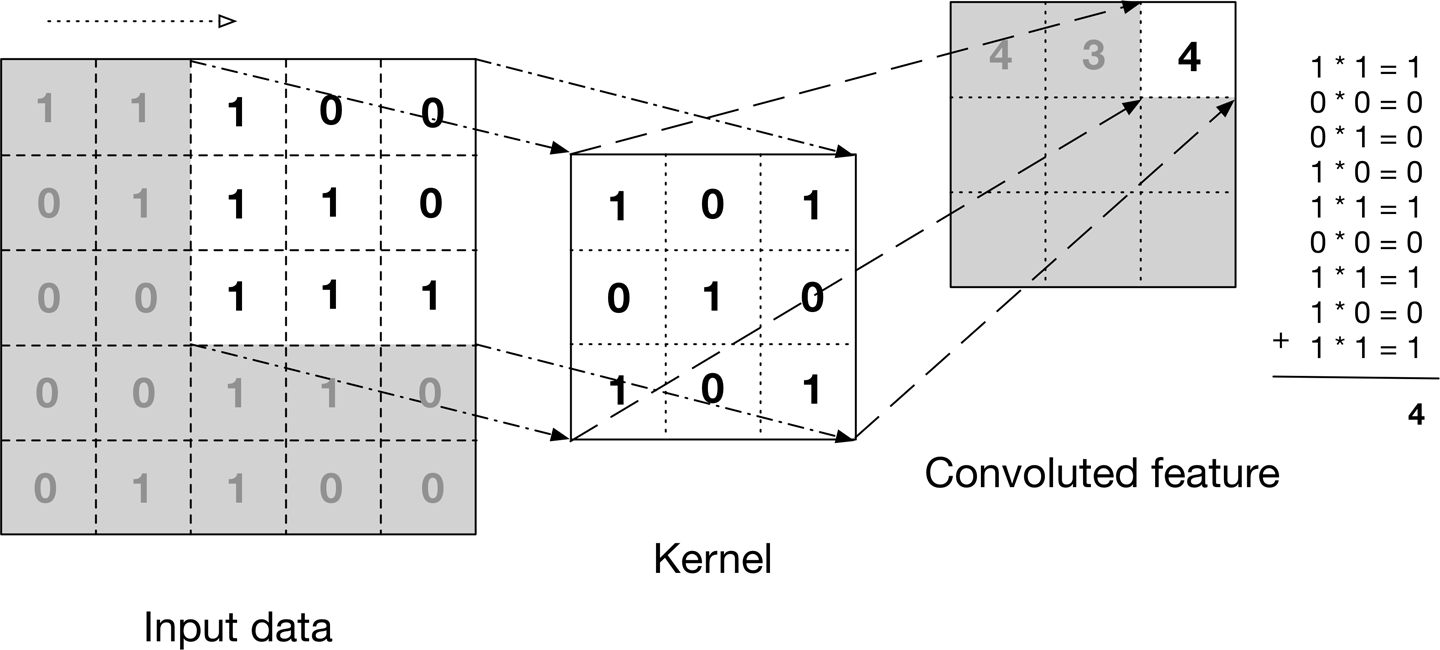
\includegraphics[width=14cm]{convolution1.png}
	\caption{Tích chập.}
\end{figure}  

Cấu trúc của CNN thường gồm ba loại lớp:
\begin{itemize}
	\item Convolution
	\item Pooling
	\item Fully connected 
\end{itemize} 

\begin{figure}[h!]
	\centering
	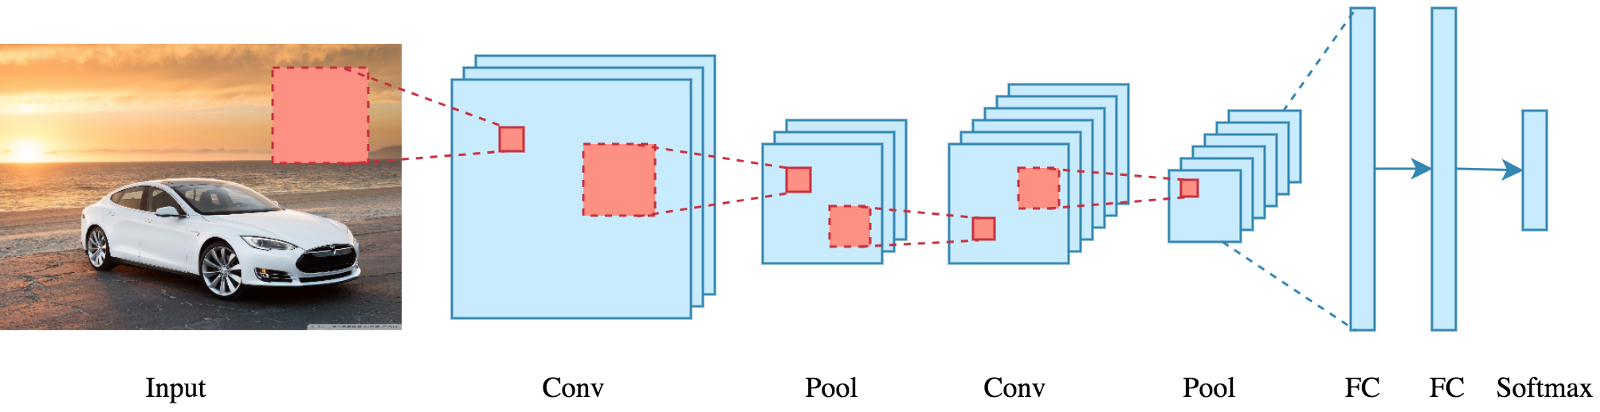
\includegraphics[width=15cm]{convo_layers.png}
	\caption{Các lớp của mô hình CNN.}
\end{figure} 

Khi đầu vào là một ảnh, mỗi lớp sẽ tạo ra các hàm kích hoạt sau đó tiếp tục được đưa vào lớp tiếp theo. Lớp đầu tiên thường sẽ trích xuất ra đặc điểm cơ bản của ảnh như các cạnh ngang và chéo. Đầu ra này sẽ được đưa vào lớp tiếp theo để xác định các góc và cạnh tổ hợp. Càng đưa vào nhiều lớp sâu hơn, ta càng tìm được các đặc điểm phức tạp như vật thể, mặt, ...\cite{web:2}.

\newpage
\subsection{Convolutional layer}
\subsubsection{a) Kernel}
Kernel là một ma trận vuông có kích thước KxK với K là các số lẻ. Ma trận X tích chập với kernal sẽ được ma trận Y.
\begin{figure}[h!]
	\centering
	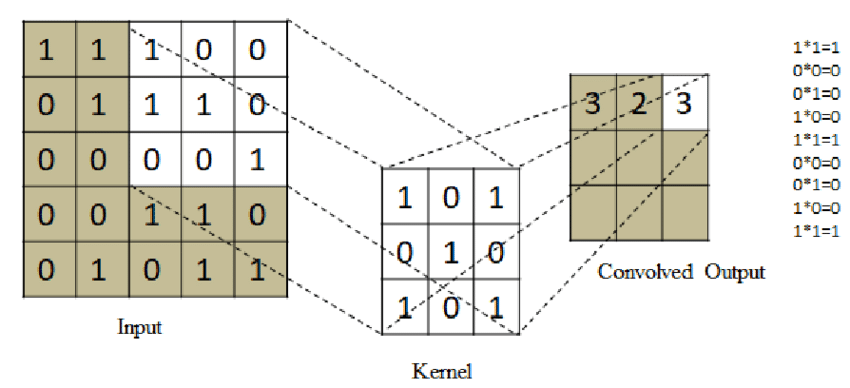
\includegraphics[width=13cm]{kernal_convo.png}
	\caption{Phép tính với kernel.}
\end{figure} 

\subsubsection{b) Padding}
Sau phép biến đổi Convolution, ma trận Y sẽ có kích thước nhỏ hơn X. Nếu muốn ma trận Y có cùng kích thước với X thì ta cần thêm giá trị 0 vào viền ngoài ma trận X trước khi thực hiện phép tính. Việc thêm viền ngoài này được gọi là Padding.

\begin{figure}[h!]
	\centering
	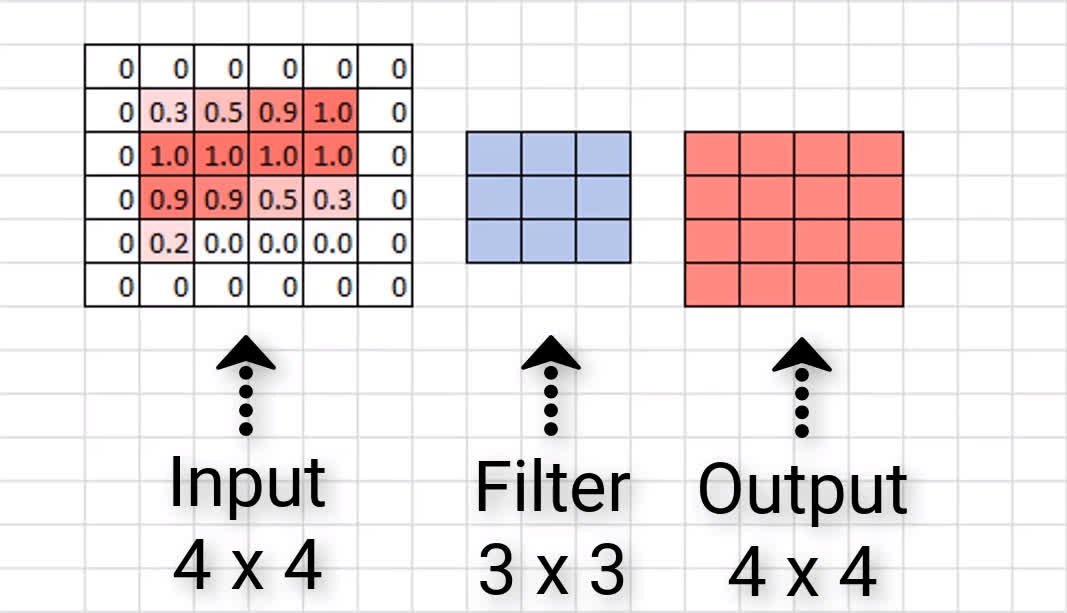
\includegraphics[width=11cm]{padding_convo.jpg}
	\caption{Thêm padding.}
\end{figure} 

\subsubsection{c) Stride}
Nếu thực hiện phép tích chập lần lượt trên các phần tử $x_{i,j}$, $x_{i,j+1}$, ... cho đến hết ma trận thì khi đó Stride là 1. Stride bằng n thì ta sẽ thực hiện phép tính trên các phần tử $x_{i,j}$, $x_{i,j+n}$, ...

\begin{figure}[h!]
	\centering
	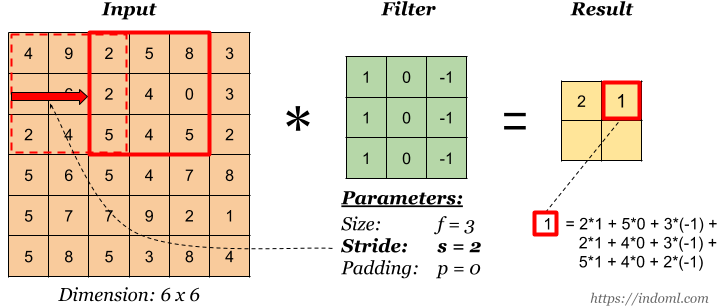
\includegraphics[width=13cm]{stride_convo.png}
	\caption{Stride = 2.}
\end{figure} 

\subsection{Polling layer}
Pooling layer thường được dùng giữa các convolutional layer, để giảm kích thước dữ liệu nhưng vẫn giữ được các thuộc tính quan trọng. Việc giảm kích thước dữ liệu giúp giảm các phép tính toán
trong model.

Bên cạnh đó, với phép pooling kích thước ảnh giảm, do đó lớp convolution học được các vùng có kích thước lớn hơn. Ví dụ như ảnh kích thước 224*224 qua pooling về 112*112 thì vùng 3*3 ở ảnh 112*112 tương ứng với vùng 6*6 ở ảnh ban đầu. Vì vậy qua các pooling thì kích thước ảnh nhỏ đi và convolutional layer sẽ học được các thuộc tính lớn hơn.

\begin{figure}[h!]
	\centering
	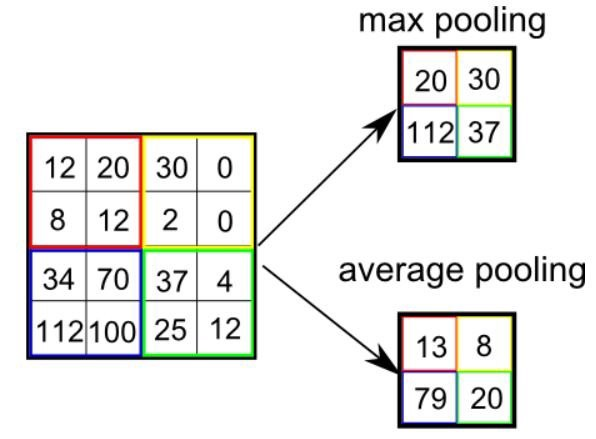
\includegraphics[width=9cm]{polling_convo.png}
	\caption{Hai loại polling.}
\end{figure} 

\newpage
\subsection{Fully connected layer}
Sau khi qua Convolution layers và Polling layers thì đầu ra vẫn là một ma trận nhiều hàng nhiều cột. Trước khi đưa dữ liệu vào lớp Fully connected ta cần phải biến đổi dữ liệu thành dạng nhiều hàng một cột.

\begin{figure}[h!]
	\centering
	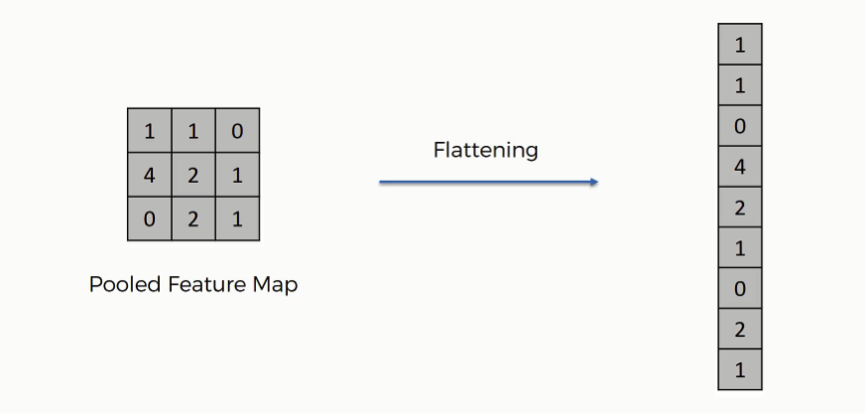
\includegraphics[width=13cm]{flatten.png}
	\caption{Flattening.}
\end{figure} 

Lớp Fully connected đề cập tới mạng nơ-ron trong đó mỗi nơ-ron áp dụng một phép biến đổi tuyến tính cho vecto đầu vào thông qua ma trận trọng số. Kết quả là tất cả đầu vào của vecto đầu vào đều có ảnh hưởng đến tất cả đầu ra của vecto đầu ra \cite{web:3}.

\begin{figure}[h!]
	\centering
	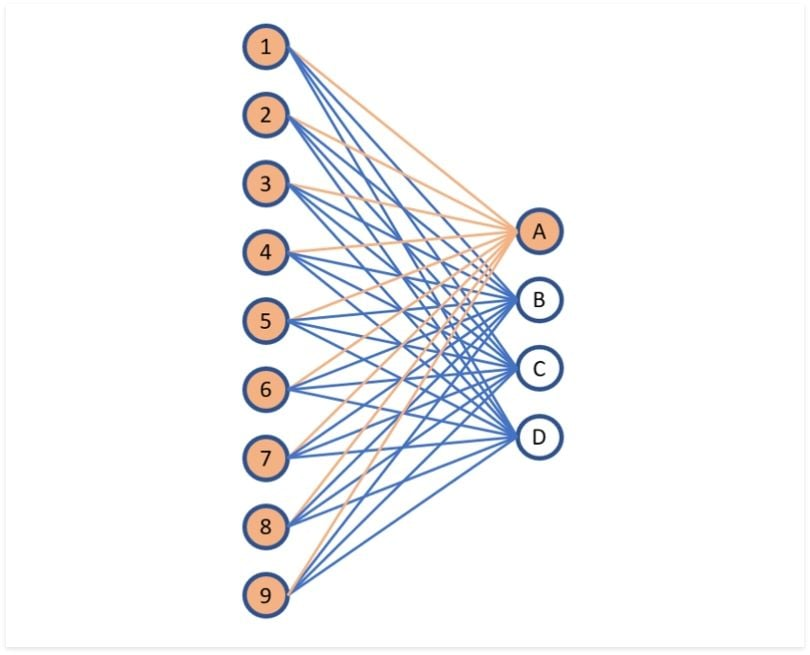
\includegraphics[width=11cm]{fully_convo.jpg}
	\caption{Fully connected layer.}
\end{figure} 

Trong quá trình đào tạo, để tránh mô hình bị overfitting (mô hình dự đoán có kết quả chính xác rất cao đối với tập dữ liệu cho trước nhưng khi áp dụng với tập dữ liệu bên ngoài thì độ chính xác giảm một cách đáng kể), một vài nơ-ron bị loại bỏ một cách ngẫu nhiên. Việc này giúp vecto đầu ra không bị phụ thuộc hoàn toàn vào giá trị của vecto đầu vào, kỹ thuật này được gọi là drop out.

\begin{figure}[h!]
	\centering
	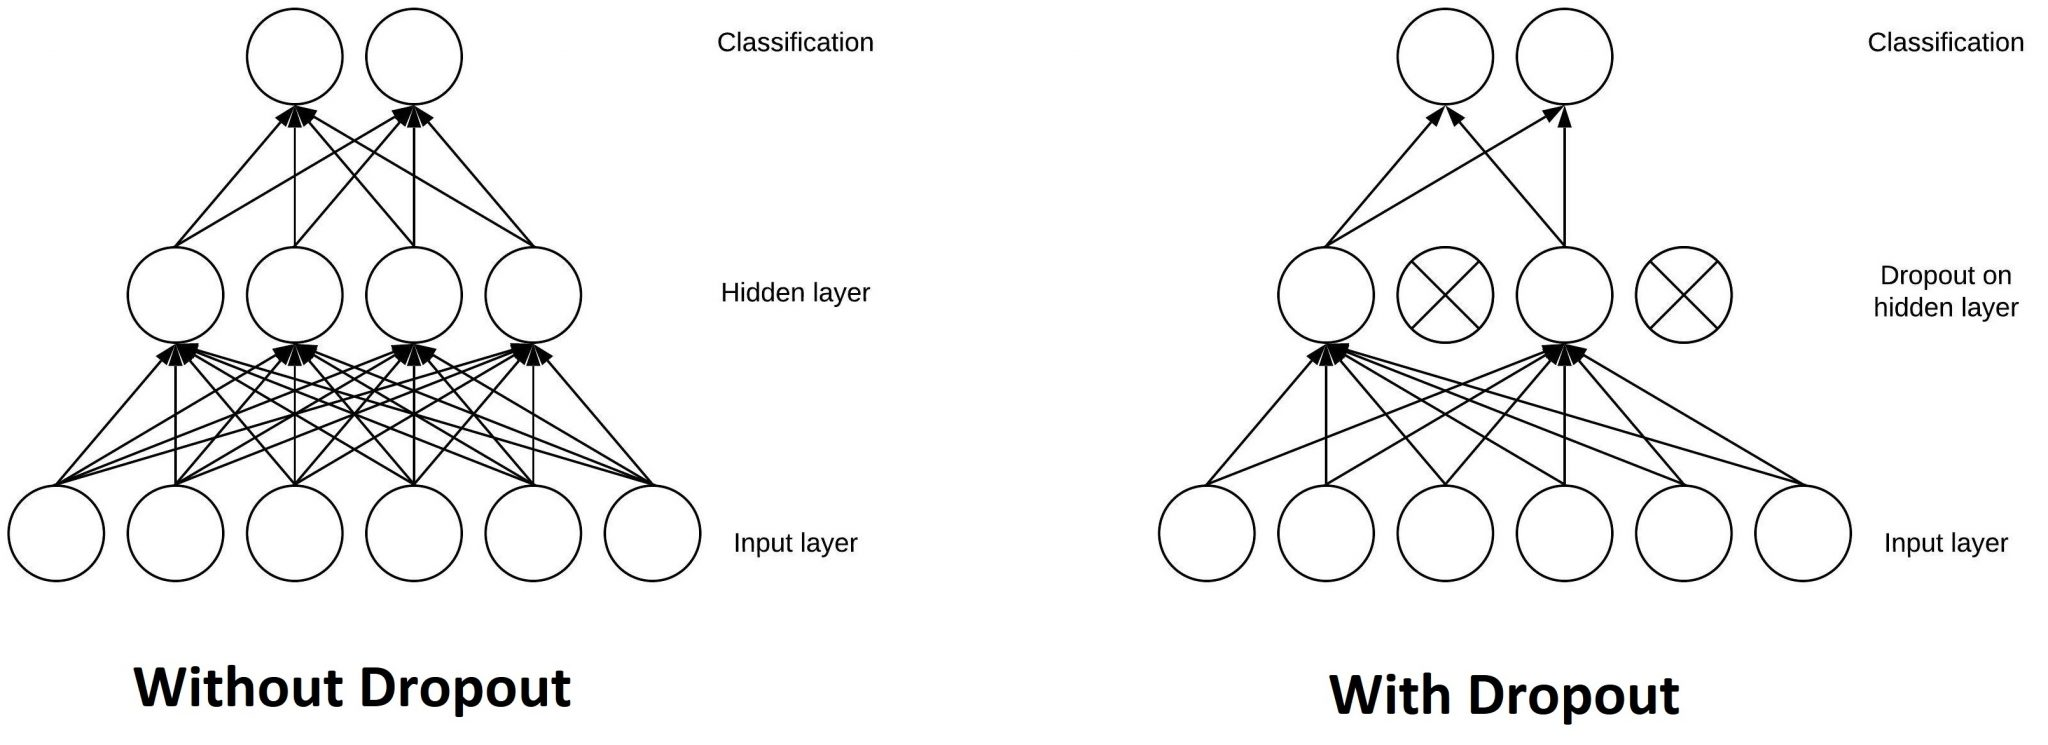
\includegraphics[width=12cm]{drop_out.jpg}
	\caption{Drop out.}
\end{figure} 

\newpage
\section{Mô hình RNN}
Như đã biết, Neural Network gồm 3 phần: Input layer, Hidden layer và Output layer. Các đầu vào và đầu ra trong mạng này đều độc lập với nhau do đó mô hình này không phù hợp với những bài toán dạng chuỗi như mô tả, hoàn thành câu,... vì những dự đoán tiếp theo sẽ phụ thuộc vào vị trí trước của nó. RNN ra đời với ý tưởng chính là để giải quyết các bài toán đó.

RNN (Recurrent Neural Network) là một kiến trúc mạng nơ-ron có khả năng xử lý và phân tích các dữ liệu tuần tự. Trong RNN, mỗi nút (hoặc đơn vị) thực hiện các phép tính trên đầu vào hiện tại và trạng thái ẩn được truyền tiếp từ đơn vị trước đó.

\begin{figure}[h!]
	\centering
	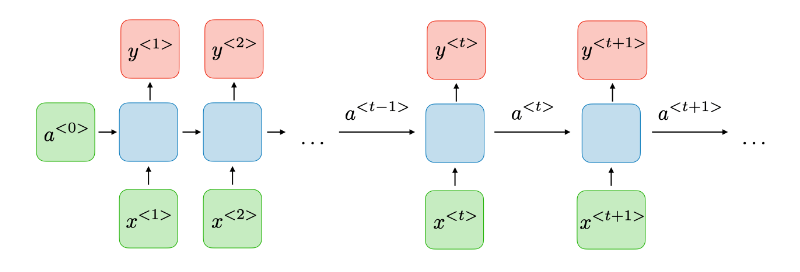
\includegraphics[width=14cm]{RNN1.png}
	\caption{Recurrent neural network.}
\end{figure} 

RNN được chia ra thành bốn loại:
\begin{itemize}
	\item One to one:
	Đây còn được gọi là mạng Neural thuần túy. Nó xử lý một kích thước cố định của đầu vào với kích thước cố định của đầu ra, nơi chúng độc lập với thông tin đầu ra trước đó. 
	\item One to many:
	Nó xử lý một kích thước cố định của thông tin làm đầu vào cung cấp một chuỗi dữ liệu làm đầu ra.
	\item Many to one:
	Bài toán có nhiều input nhưng chỉ có 1 output, ví dụ bài toán phân loại hành động trong video, input là nhiều ảnh (frame) tách ra từ video, ouptut là hành động trong video.
	\item Many to many:
	Bài toán có nhiều input và nhiều output, ví dụ bài toán dịch từ tiếng Anh sang tiếng Việt, input là 1 câu gồm nhiều chữ: “I love Vietnam” và output cũng là 1 câu gồm nhiều chữ “Tôi yêu Việt Nam”.
\end{itemize}

\begin{figure}[h!]
	\centering
	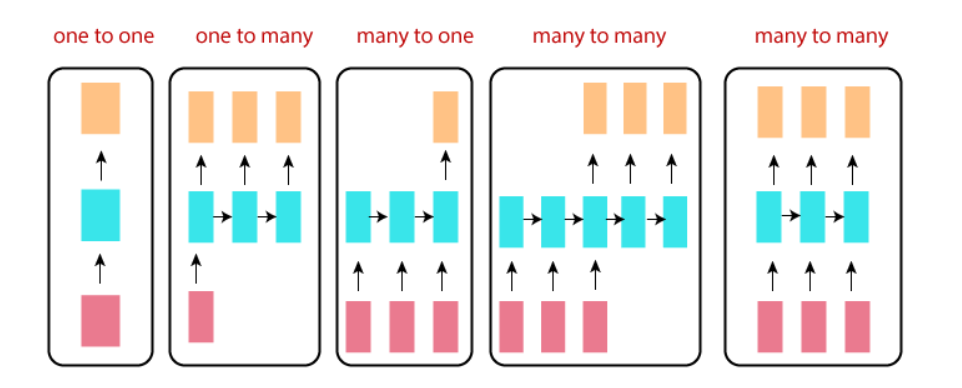
\includegraphics[width=13cm]{cacRNN.png}
	\caption{Các loại RNN.}
\end{figure} 

Tuy nhiên mô hình RNN cũng tồn tại những hạn chế rõ ràng \cite{web:5}:
\begin{itemize}
	\item RNN có nhiệm vụ đưa thông tin đi kịp thời. Tuy nhiên, việc truyền tất cả các thông tin này là một việc khá khó khăn bởi thời gian quá dài. Điều đó dẫn đến RNN có thể gặp phải vanishing gradient (hệ số phản hồi không thể thay đổi khi các trạng thái mới đi qua mô hình). Việc này đồng nghĩa với việc mô hình không thể học được từ thông tin do đó kết quả đưa ra sẽ bị sai.
	\item Không thể mô hình hóa các thông tin dài hạn.
	\item RNN yêu cầu đầu vào mỗi chuỗi có độ dài bằng nhau do đó khó khăn trong việc xử lý các chuỗi có độ dài khác nhau. 
\end{itemize}

\newpage
\section{Mô hình LSTM}
Xuất phát từ những nhược điểm kể trên của RNN truyền thống, mô hình LSTM (Long Short – Term Memory) đã được ra đời. Dù mô hình LSTM có những kết nối phản hồi như mô hình RNN, nhưng quá trình xử lý không chỉ các điểm dữ liệu đơn lẻ mà là toàn bộ chuỗi dữ liệu. Từ đó kết quả trở lên lý tưởng hơn để xử lý và dự đoán dữ liệu, LSTM có nhiều ứng dụng trong nhận dạng chữ viết tay, nhận diện giọng nói, phát hiện giọng nói, trò chơi,...\cite{hochreiter1997long}

\subsection{Short term và Long term memory}
Short term memory là quá trình học từ những trạng thái được lưu trữ thông tin của layer trước tới layer sau khi thông tin đó được mang qua state nhất định. Nó là giá trị lưu trữ để tính toán đầu ra dự đoán đối với giá trị input. Short term memory của mô hình RNN sẽ tiếp tục liện tục qua nhiều state và khó kiểm soát và gặp vấn đề.

Long term memory là quá trình xác định thông tin đi xa hơn sau hàng ngàn state và sẽ được sử dụng khi cần. Giá trị long term memory sẽ được lưu trữ mới mỗi khi mộtshort term memory tính toán ra state tiếp theo của layer.

Để không xảy ra hiện tượng vanishing gradient, hàm kích hoạt được sử dụng là tanh và sigmoid. Giá trị đầu ra của hàm tanh bị giới hạn từ -1 < y < 1; đầu ra của hàm sigmoid giới hạn từ 0 < y < 1 sẽ điều chỉnh đầu ra như một hàm xác suất để dự đoán giống như các bài toán của Machine Learning. Kể cả đầu vào là một hình ảnh với ma trận hệ số màu thì các giá trị vẫn sẽ cùng giữ các đặc trưng (tỷ lệ chênh lệch) khi đi qua mô hình.

\newpage
\subsection{Cấu trúc mô hình LSTM}
Cấu trúc của mô hình LSTM bao gồm một chuỗi các đơn vị lặp lại gọi là LSTM cells.

\begin{figure}[h!]
	\centering
	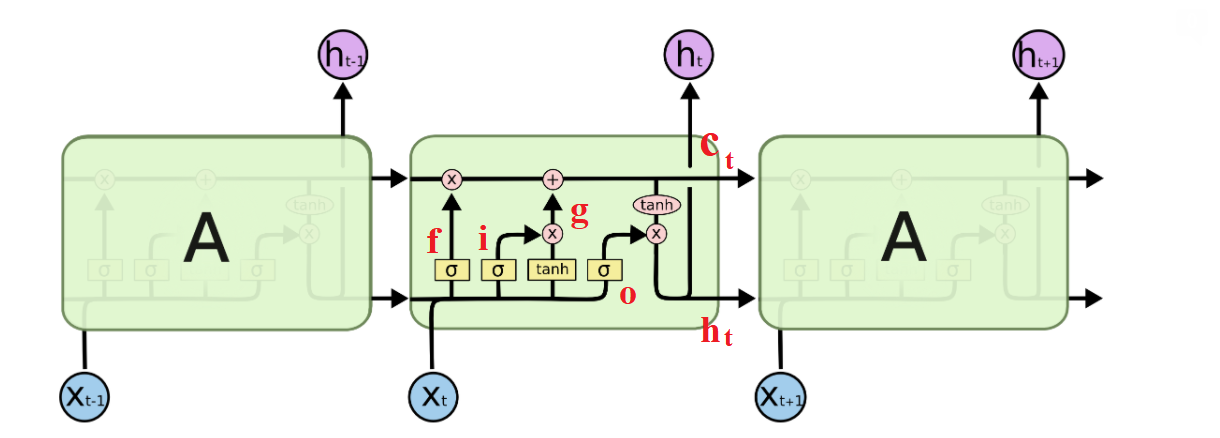
\includegraphics[width=13cm]{LSTM.png}
	\caption{Mô hình LSTM.}
\end{figure} 

Mỗi LSTM cell bao gồm 3 cổng chính \cite{web:6}: 
\begin{itemize}
	\item Forget gate (f):
	Thực hiện việc quyết định thông tin nào từ trước đó sẽ được lưu lại trong bộ nhớ.
	\item Input gate (i):
	Thực hiện việc quyết định những thông tin mới nào sẽ được lưu lại trong bộ nhớ dài hạn.
	\item Output gate (o):
	Thực hiện xem thông tin nào được truyền ra ngoài để phục vụ cho mục đích dự đoán.
\end{itemize}

Ngoài ra thành phần của LSTM cell còn có cell state ($c_t$). Là bộ nhớ trong của LSTM, nó là tổng hợp của bộ nhớ trước $c_{t-1}$ đã được lọc qua Forget gate, cộng với trạng thái ẩn g đã được lọc bởi Input gate sẽ mang thông tin nào quan trọng truyền đi xa hơn và sẽ được dùng khi cần. Đây chính là long term memory.

Cơ chế hoạt động đặc biệt và cổng (gate) của LSTM giúp mô hình có khả năng lưu trữ thông tin dài hạn và xử lý hiệu quả các chuỗi có độ dài khác nhau, giúp khắc phục được các nhược điểm của RNN. Tuy nhiên LSTM vẫn tồn tại điểm yếu là độ phức tạp của nó khiến thời gian xử lý lớn hơn nhiều so với mô hình RNN thông thường. 
\chapter{XÂY DỰNG MÔ HÌNH}

\label{Chapter3}
\section{Xây dựng mô hình}

\section{BLEU Score}
BLEU (BiLingual Evaluation Understudy) là một phương pháp sử dụng trong dịch máy (Machine translation). BLEU đánh giá một câu thông qua việc so sánh khớp giữa câu máy sinh ra (candidate) và câu mẫu (preference), giá trị của đánh giá từ khoảng 0 tới 1. Giá trị 0 thể hiện việc đầu ra sai hoàn toàn và giá trị 1 thể hiện việc đúng hoàn toàn. Thông thường giá trị BLEU đạt trên 40\% đã được coi là rất tốt \cite{lavie2010evaluating}.

BLEU đánh giá mô tả thông qua \cite{papineni2002bleu}:
\begin{itemize}
	\item Adequacy: Mô tả đầy đủ thông tin trong ảnh
	\item Fluency: Đúng ngữ pháp, cấu trúc câu
\end{itemize}

\begin{figure}[h!]
	\centering
	\subfigure{
		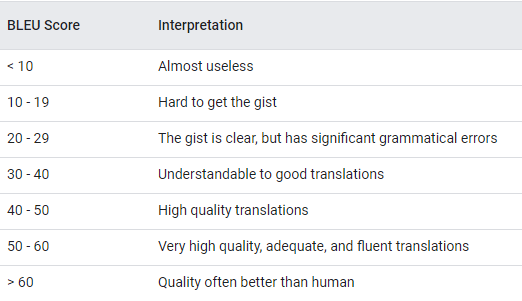
\includegraphics[width=14cm]{BLEU.png}}
	\subfigure{
		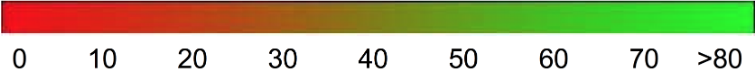
\includegraphics[width=14cm]{BLEU_scale.png}}         
	\caption{Đánh giá BLEU.}
\end{figure}

Đánh giá BLEU được tính toán như sau:
\begin{figure}[h!]
	\centering
	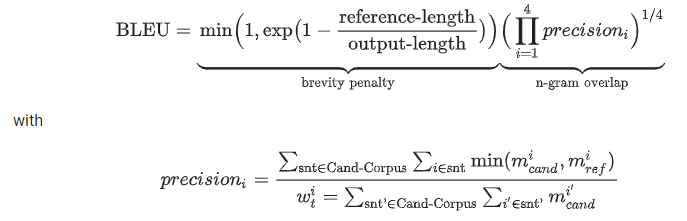
\includegraphics[width=15cm]{BLEU_cal.png}
	\caption{Tính toán đánh giá BLEU.}
\end{figure} 

Công thức tính bao gồm hai phần \cite{web:10}:
\begin{itemize}
	\item Brevity penalty:
	Dùng để hạn chế việc đánh giá tốt cho các câu ngắn và kém cho các câu dài hơn.
	\item N-gram overlap:
	Hoạt động như một hàm tính độ chính xác của đầu ra.
\end{itemize}

trong đó
\begin{itemize}
	\item $m_{cand}^i$: Số lượng i-gram trong candidate khớp với reference.
	\item $m_{ref}^i$: Số lượng i-gram trong reference.
	\item $w_{t}^i$: Tổng số i-gram trong candidate.
\end{itemize}
\section{Nhận xét kết quả}
%\chapter*{Kết luận} % Tên của chương
\addcontentsline{toc}{chapter}{Kết luận} % Thêm tên chương vào mục lục

\label{Chapter_end}

Sau một thời gian nghiên cứu về MQTT và các ứng dụng liên quan tôi đã thu được một số kết quả như sau.

Đã tìm hiểu được giao thức MQTT, trên cơ sở của giao thức này đã xây dựng thành công hệ thống thu thập và hiển thị dữ liệu nhiệt độ, độ ẩm. Hệ thống này bao gồm phần cứng sau:
\begin{itemize}
	\item Hai board ESP8266 với vai trò là publisher và subcriber, xử lí dữ liệu nhận được từ cảm biến, gửi cũng như nhận dữ liệu thông qua broker trung gian là HiveMQ.
	\item Cảm biến DHT11 thu thập dữ liệu nhiệt độ, độ ẩm từ môi trường bên ngoài.
\end{itemize}

Mô hình của hệ thống có thể triển khai và ứng dụng nhiều vào các lĩnh vực khác nhau.  Tuy nhiên, để nâng cao tính bảo mật thì mô hình cần dùng một broker trả phí hoặc là tự phát triển broker thay vì sử dụng broker miễn phí như đã trình bày. Một số broker trả phí có thể kể tới là: Azure, AWS, CloudMQTT,...

Kết quả nghiên cứu của tiểu luận này rất hữu ích cho những người mới tiếp cận với IoT, đặc biệt là sử dụng giao thức MQTT cần tài liệu tham khảo. 
%\include{Chapters/Chapter5} 

%----------------------------------------------------------------------------------------
%	(KHÔNG CHỈNH SỬA PHẦN NÀY)
%
%	PHẦN 13: TÀI LIỆU THAM KHẢO
%----------------------------------------------------------------------------------------

\begin{spacing}{1.15}
	\printbibliography[heading=bibintoc, title=Tài liệu tham khảo] % In ra tài liệu tham khảo
\end{spacing}

%----------------------------------------------------------------------------------------
%	PHẦN 14: PHỤ LỤC (THESIS CONTENT - APPENDICES)
%----------------------------------------------------------------------------------------

\appendix % Nói với LaTeX rằng những chương về sau được tính là phụ lục

% Hãy thêm những phụ lục (appendix) của khóa luận/tiểu luận vào thư mục Appendices
% Hãy bỏ chú thích những dòng nếu bạn đã bổ sung những phụ lục vào

% Phụ lục A

\chapter{MÃ NGUỒN} % Tên của phụ lục

\label{AppendixA} % Để trích dẫn chương này ở chỗ nào đó trong bài, hãy sử dụng lệnh \ref{AppendixA} 
\begin{lstlisting}

\end{lstlisting}







%% Phụ lục B

\chapter{Liệt kê source code} % Tên của phụ lục

\label{AppendixB} % Để trích dẫn chương này ở chỗ nào đó trong bài, hãy sử dụng lệnh \ref{AppendixB} 

%----------------------------------------------------------------------------------------

\section{Ví dụ liệt kê code ngôn ngữ C/C++}

Code tính khoảng thời gian giữa hai thời điểm cho trước. Lệnh thực hiện là:
\begin{Verbatim}
\lstinputlisting{"Code/TimeDiff.cpp"}
\end{Verbatim}

File \file{TimeDiff.cpp}:
%https://www.programiz.com/cpp-programming/examples/time-structure
\lstinputlisting{"Code/TimeDiff.cpp"}


%----------------------------------------------------------------------------------------

\section{Ví dụ liệt kê thông tin ở terminal (console/command prompt) từ file text}

Sau khi biên dịch và chạy file \file{TimeDiff.cpp}, kết quả chạy được hiển thị ở terminal. Trong trường hợp bạn muốn liệt kê quá trình chạy, bạn có thể copy đoạn text ở terminal vào một file text, và liệt kê chúng chẳng hạn như:
\begin{Verbatim}
\lstinputlisting[style=console]{"Code/TimeDiff.txt"}
\end{Verbatim}

File \file{TimeDiff.txt}:
\lstinputlisting[style=console]{"Code/TimeDiff.txt"}


%----------------------------------------------------------------------------------------

\section{Ví dụ liệt kê code ngôn ngữ Python}

Code tính mã hash của một file. Lệnh thực hiện là:
\begin{Verbatim}
\lstinputlisting[style=codePython]{"Code/Hash.py"}
\end{Verbatim}

File \file{Hash.py}:
%https://www.programiz.com/python-programming/examples/hash-file
\lstinputlisting[style=codePython]{"Code/Hash.py"}


%----------------------------------------------------------------------------------------

\section{Ví dụ liệt kê code ngôn ngữ Matlab}

Code biểu diễn bản chất và sai số của phương pháp Euler và Heun trong việc giải phương trình vi phân. Lệnh thực hiện là:
\begin{Verbatim}
\lstinputlisting[style=codeMatlab]{"Code/EulerVisualization.m"}
\end{Verbatim}

File \file{EulerVisualization.m}:
\lstinputlisting[style=codeMatlab]{"Code/EulerVisualization.m"}


%----------------------------------------------------------------------------------------

\section{Ví dụ liệt kê file text thông thường (plain text)}

Một file text lưu giữ thông số của một lần chạy mô phỏng động học phân tử. Lệnh thực hiện là:
\begin{Verbatim}
\lstinputlisting[style=plaintext]{"Code/minim.mdp"}
\end{Verbatim}

File \file{minim.mdp}:
\lstinputlisting[style=plaintext]{"Code/minim.mdp"}




%\include{Appendices/AppendixC}

%----------------------------------------------------------------------------------------

\end{document} 
%----------------------------------------------------------------------------------------------------------------------------------------
